\mode*
\begin{frame}[label=tendencias]
  \tendenciasTime
  \frametitle{Trabajos relevantes de los \'ultimos 8 a\~nos}
  \framesubtitle{Tendencias mundiales en investigaci\'on}
  \begin{columns}[T]
    \begin{column}{2.0cm}
      \setbeamercovered{transparent}
      \uncover<2>{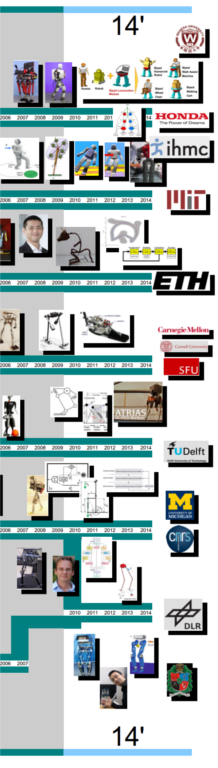
\includegraphics[height=7.5cm]{../images/TimeLineTendencias_0.png}}
    \end{column}
    \begin{column}{5.0cm}
      \only<1-3>{
        \begin{center}
          \only<1>{\textbf{\textcolor{redun}{Universidad de Waseda}}}%
          \only<2-3>{\textbf{\textcolor{blueun}{Universidad de Waseda}}}
          \begin{center}
            
\includegraphics[height=1.5cm]{../images/WasedaLogo.png}\\
          \end{center}
          \only<2-3>{\hspace{1.5cm}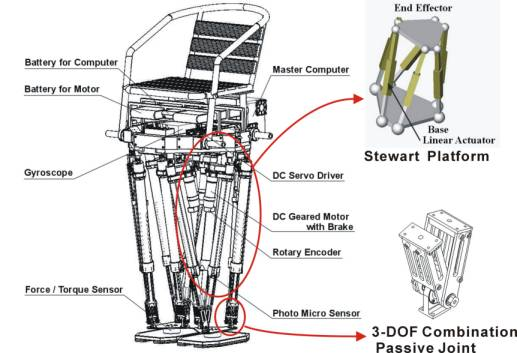
\includegraphics[height=3.8cm]{../images/WasedaTendencias.png}}
        \end{center}
      }
      \only<4-6>{
        \begin{center}
          \only<4>{\textbf{\textcolor{redun}{Honda Research Institute\\\& IHMC}}}%
          \only<5-6>{\textbf{\textcolor{blueun}{Honda Research Institute\\\& IHMC}}}
          \begin{center}
            
\includegraphics[height=0.7cm]{../images/HondaLogo.png}\quad
            
\includegraphics[height=0.7cm]{../images/IHMCLogo.png}
          \end{center}
          \only<5-6>{\hspace{1.8cm}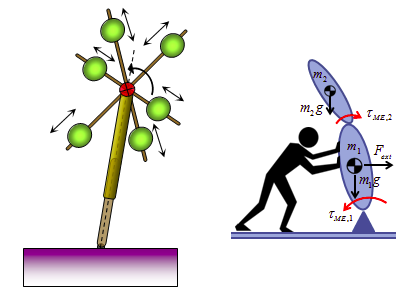
\includegraphics[height=4.0cm]{../images/HondaTendencias.png}}
        \end{center}
      }
      \only<7-9>{
        \begin{center}
          \only<7>{\textbf{\textcolor{redun}{Aldebaran Robotics}}}%
          \only<8-9>{\textbf{\textcolor{blueun}{Aldebaran Robotics}}}
          \begin{center}
            
\includegraphics[height=1.0cm]{../images/AldebaranLogo.png}\\
          \end{center}
          \only<8-9>{\vspace{0.5cm}\hspace{0.3cm}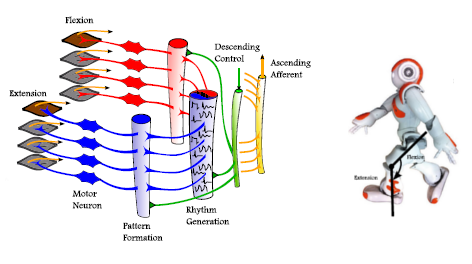
\includegraphics[height=4.0cm]{../images/AldebaranTendencias.png}}
        \end{center}
      }
      \only<10-12>{
        \begin{center}
          \only<10>{\textbf{\textcolor{redun}{MIT\\Robot Locomotion Group}}\\}%
          \only<11-12>{\textbf{\textcolor{blueun}{MIT\\Robot Locomotion Group}}\\}
          \begin{center}
            
\includegraphics[height=1.0cm]{../images/MITLogo.png}
          \end{center}
          \only<11-12>{\vspace{0.5cm}\hspace{1.5cm}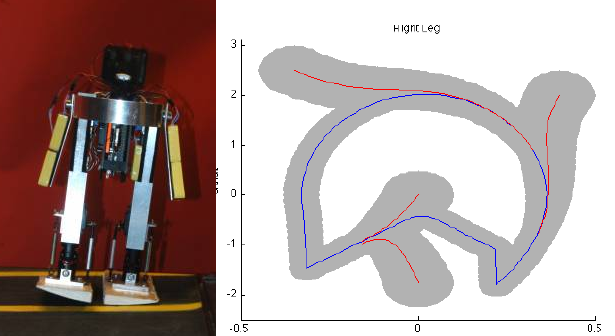
\includegraphics[height=3.0cm]{../images/MITTendencias.png}}
        \end{center}
      }
      \only<13-15>{
        \begin{center}
          \only<13>{\textbf{\textcolor{redun}{ETH-BIRLab}}\\}%
          \only<14-15>{\textbf{\textcolor{blueun}{ETH-BIRLab}}\\}
          \begin{center}
            
\includegraphics[height=1.0cm]{../images/ETHLogo.png}
          \end{center}
          \only<14-15>{\vspace{0.5cm}\hspace{1.5cm}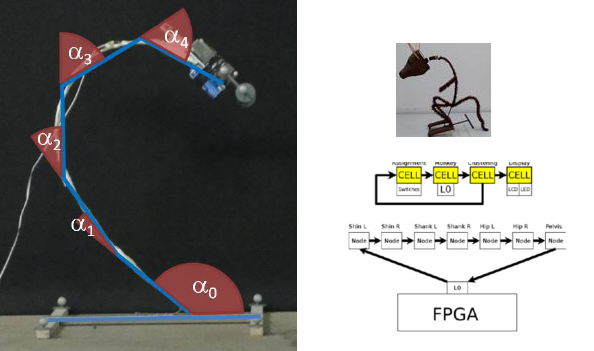
\includegraphics[height=4.0cm]{../images/ETHTendencias.png}}
        \end{center}
      }
      \only<16-18>{
        \begin{center}
          \only<16>{\textbf{\textcolor{redun}{CMU - Biorobotics and \\ CU - Locomotion Labs}}}%
          \only<17-18>{\textbf{\textcolor{blueun}{CMU - Biorobotics and \\ CU - Locomotion Labs}}}
          \begin{center}
            
\includegraphics[height=0.7cm]{../images/CMULogo.png}\\
            
\includegraphics[height=0.7cm]{../images/CornellULogo.png}
          \end{center}
          \only<17-18>{\vspace{0.1cm}\hspace{1.5cm}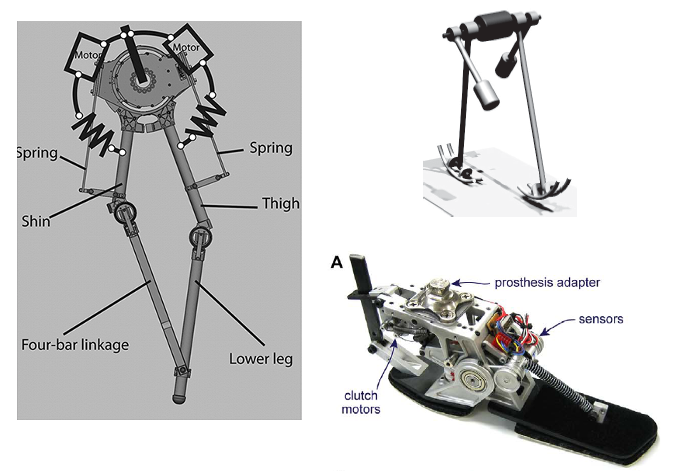
\includegraphics[height=3.5cm]{../images/CMUCornellTendencias.png}}
        \end{center}
      }
      \only<19-21>{
        \begin{center}
          \only<19>{\textbf{\textcolor{redun}{Delft University-DBL Lab}}\\}%
          \only<20-21>{\textbf{\textcolor{blueun}{Delft University-DBL Lab}}\\}
          \begin{center}
            
\includegraphics[height=1.0cm]{../images/DelftLogo.png}\\
          \end{center}
          \only<20-21>{\vspace{0.1cm}\hspace{2.5cm}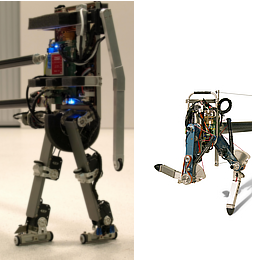
\includegraphics[height=4.0cm]{../images/DelftTendencias.png}}
        \end{center}
      }
      \only<22-24>{
        \begin{center}
          \only<22>{\textbf{\textcolor{redun}{Gottingen University}}}%
          \only<23-24>{\textbf{\textcolor{blueun}{Gottingen University}}}
          \begin{center}
            
\includegraphics[height=1.5cm]{../images/GottingenULogo.png}
          \end{center}
          \only<23-24>{\vspace{0.1cm}\hspace{2.0cm}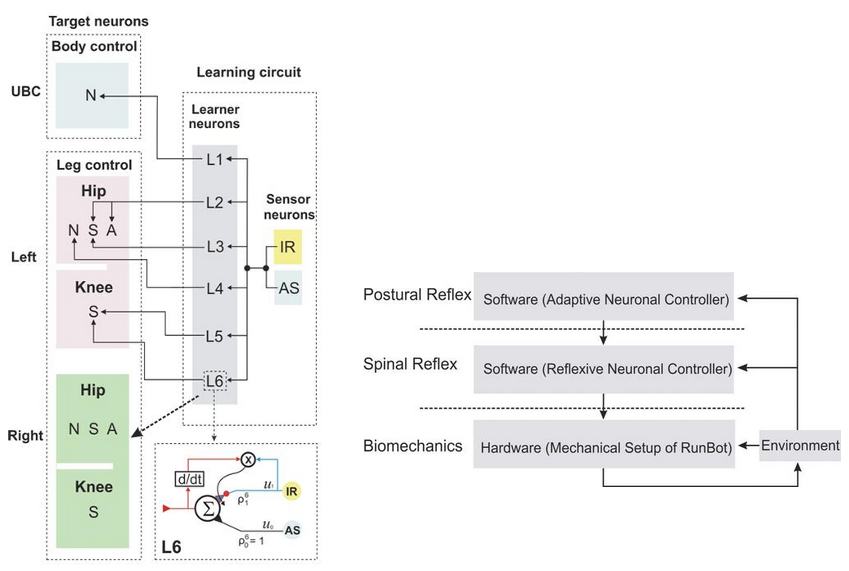
\includegraphics[height=3.5cm]{../images/GottingenUTendencias.png}}
        \end{center}
      }
      \only<25-27>{
        \begin{center}
          \only<25>{\textbf{\textcolor{blueun}{CNRS}}}%
          \only<26-27>{\textbf{\textcolor{blueun}{CNRS}}}
          \begin{center}
            
\includegraphics[height=2.0cm]{../images/CNRSLogo.png}\\
          \end{center}
          \only<26-27>{\vspace{0.1cm}\hspace{2.0cm}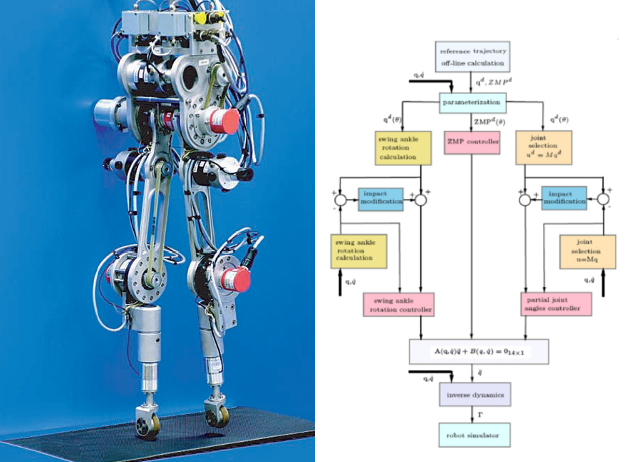
\includegraphics[height=3.5cm]{../images/CNRSTendencias.png}}
        \end{center}
      }
      \only<28-30>{
        \begin{center}
          \only<28>{\textbf{\textcolor{blueun}{DLR-biped}}}%
          \only<29-30>{\textbf{\textcolor{blueun}{DLR-biped}}}
          \begin{center}
            
\includegraphics[height=1.0cm]{../images/DLRLogo.png}\\
          \end{center}
          \only<29-30>{\vspace{0.1cm}\hspace{1.0cm}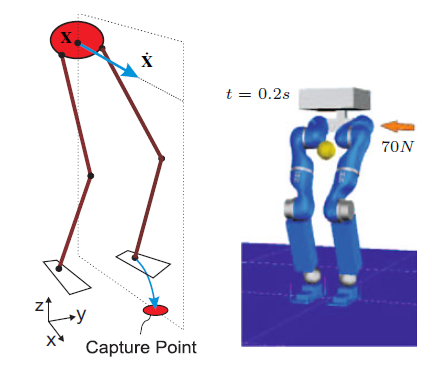
\includegraphics[height=4.0cm]{../images/DLRTendencias.png}}
        \end{center}
      }
    \end{column}
    \begin{column}{3.5cm}
      \only<3>{
        \begin{center}
          \vspace{1.3cm}
          \textbf{\textcolor{redun}{Tendencias}}
          \begin{itemize}\scriptsize
          \item Rob\'otica paralela
          \end{itemize}
          % \includegraphics[height=1.0cm]{../images/WasedaTendencias01.png}            
        \end{center}
      }
      \only<6>{
        \begin{center}
          \vspace{1.3cm}
          \textbf{\textcolor{redun}{Tendencias}}
          \begin{itemize}\scriptsize
          \item Control
          \item Efectos del Torso
          \end{itemize}
        \end{center}
      }
      \only<9>{
        \begin{center}
          \vspace{1.3cm}
          \textbf{\textcolor{redun}{Tendencias}}
          \begin{itemize}\scriptsize
          \item CPG, ANN
          \item AI, Aprendizaje
          \end{itemize}
        \end{center}
      }
      \only<12>{
        \begin{center}
          \vspace{1.3cm}
          \textbf{\textcolor{redun}{Tendencias}}
          \begin{itemize}\scriptsize
          \item Control:{\tiny LQR-trees, SVM}
          \item Rob\'otica subactuada
          \end{itemize}
        \end{center}
      }
      \only<15>{
        \begin{center}
          \vspace{1.3cm}
          \textbf{\textcolor{redun}{Tendencias}}
          \begin{itemize}\scriptsize
          \item Bajo costo
          \item CPG, SVM
          \item BAN
          \end{itemize}
        \end{center}
      }
      \only<18>{
        \begin{center}
          \vspace{1.3cm}
          \textbf{\textcolor{redun}{Tendencias}}
          \begin{itemize}\scriptsize
          \item Balanceo, torso, SLIP
          \item Talon y tobillo
          \item Modelos Masa-resorte
          \end{itemize}
        \end{center}
      }
      \only<21>{
        \begin{center}
          \vspace{1.3cm}
          \textbf{\textcolor{redun}{Tendencias}}
          \begin{itemize}\scriptsize
          \item Running robot
          \item Air Muscles and DC motors
          \item Balance
          \end{itemize}
        \end{center}
      }
      \only<24>{
        \begin{center}
          \vspace{1.3cm}
          \textbf{\textcolor{redun}{Tendencias}}
          \begin{itemize}\scriptsize
          \item Aprendizaje de m\'aquina
          \item Control adaptativo
          \item Running Mode
          \end{itemize}
        \end{center}
      }
      \only<27>{
        \begin{center}
          \vspace{1.3cm}
          \textbf{\textcolor{redun}{Tendencias}}
          \begin{itemize}\scriptsize
          \item Control y trayectoria
          \item Running Mode
          \end{itemize}
        \end{center}
      }
      \only<30>{
        \begin{center}
          \vspace{1.3cm}
          \textbf{\textcolor{redun}{Tendencias}}
          \begin{itemize}\scriptsize
          \item Capture Points
          \item Control de torque de cuerpo completo
          \item Agarre de cuerpo completo
          \end{itemize}
        \end{center}
      }
    \end{column}
  \end{columns}
\end{frame}
